\chapter{Lampiran Pengujian Eksperimental}
\label{lamp:B}

\section{Kuesioner}
\label{sec:survey}
Kuesioner diawali dengan pertanyaan :
\begin{figure}[H]
	\centering  
	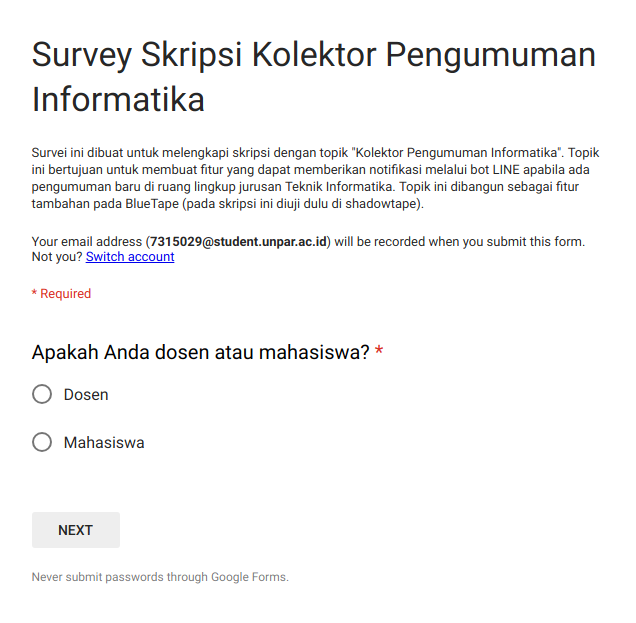
\includegraphics[scale=0.5]{./Survey-Kuesioner/Q0.png}  
	\caption[Kuesioner bagian pertama]{Kuesioner bagian pertama} 
	\label{fig:q0} 
\end{figure}

Apabila responden memilih "Dosen", maka responden akan dialihkan ke bagian Dosen (Lampiran \ref{subsec:survey-dosen}). Apabila responden memilih "Mahasiswa", maka responden akan dialihkan ke bagian Mahasiswa (Lampiran \ref{subsec:survey-mahasiswa}). Responden wajib mengisi semua pertanyaan di kuesioner ini kecuali pertanyaan saran.

\subsection{Dosen}
\label{subsec:survey-dosen}
\begin{figure}[H]
	\centering  
	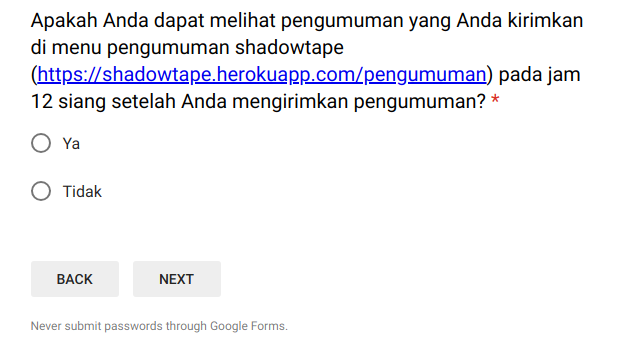
\includegraphics[scale=0.5]{./Survey-Kuesioner/Q1-D1.png}  
	\caption[Kuesioner bagian Dosen pertanyaan pertama]{Kuesioner bagian Dosen pertanyaan pertama} 
	\label{fig:q1-d1} 
\end{figure}

Apabila responden memilih jawaban "Ya" pada pertanyaan pertama (Gambar~\ref{fig:q1-d1}), maka responden akan dialihkan ke pertanyaan kedua (Gambar~\ref{fig:q1-d2}). Apabila responden memilih jawaban "Tidak", maka responden akan dialihkan ke bagian \textit{System Usability Scale} dan Saran (Lampiran \ref{subsec:final}) dan Saran (Gambar~\ref{subsec:final}). 

\begin{figure}[H]
	\centering  
	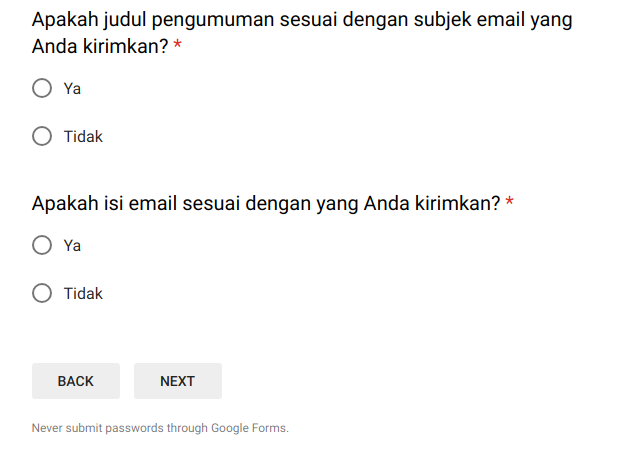
\includegraphics[scale=0.5]{./Survey-Kuesioner/Q1-D2.png}  
	\caption[Kuesioner bagian Dosen pertanyaan kedua dan ketiga]{Kuesioner bagian Dosen pertanyaan kedua dan ketiga} 
	\label{fig:q1-d2} 
\end{figure}

Apabila responden memilih jawaban "Ya" pada pertanyaan ketiga (pertanyaan kedua di Gambar~\ref{fig:q1-d1}), maka responden akan dialihkan ke pertanyaan keempat (Gambar~\ref{fig:q1-d3}). Apabila responden memilih jawaban "Tidak", maka responden akan dialihkan ke bagian \textit{System Usability Scale} dan Saran (Gambar~\ref{subsec:final}). 

\begin{figure}[H]
	\centering  
	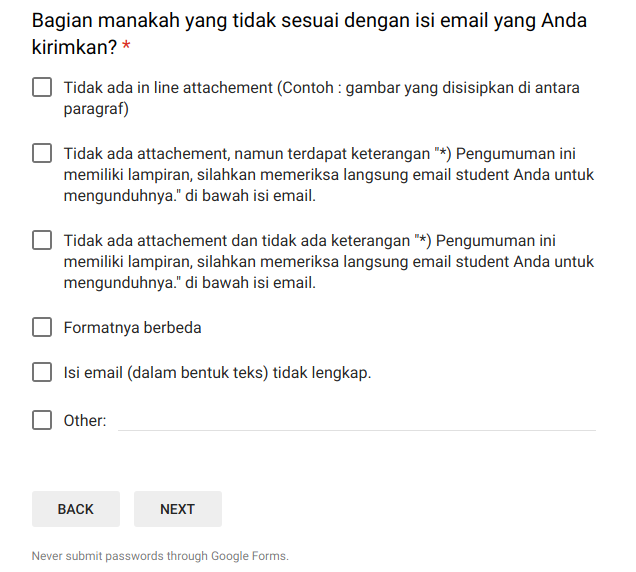
\includegraphics[scale=0.5]{./Survey-Kuesioner/Q1-D3.png}  
	\caption[Kuesioner bagian Dosen pertanyaan keempat]{Kuesioner bagian Dosen pertanyaan keempat} 
	\label{fig:q1-d3} 
\end{figure}

Apapun jawaban responden pada pertanyaan keempat (Gambar~\ref{fig:q1-d3}), responden akan dialihkan ke bagian \textit{System Usability Scale} dan Saran (Gambar~\ref{subsec:final}).

\subsection{Mahasiswa}
\label{subsec:survey-mahasiswa}
\begin{figure}[H]
	\centering  
	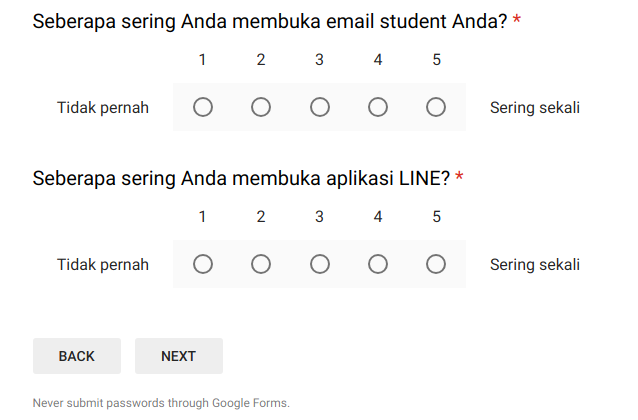
\includegraphics[scale=0.5]{./Survey-Kuesioner/Q1-M1.png}  
	\caption[Kuesioner bagian Mahasiswa pertanyaan pertama dan kedua]{Kuesioner bagian Mahasiswa pertanyaan pertama dan kedua} 
	\label{fig:q1-m1} 
\end{figure}

Apapun jawaban responden pada pertanyaan pertama dan kedua(Gambar~\ref{fig:q1-m1}), responden akan dialihkan ke pertanyaan kedua (Gambar~\ref{fig:q1-m2}).

\begin{figure}[H]
	\centering  
	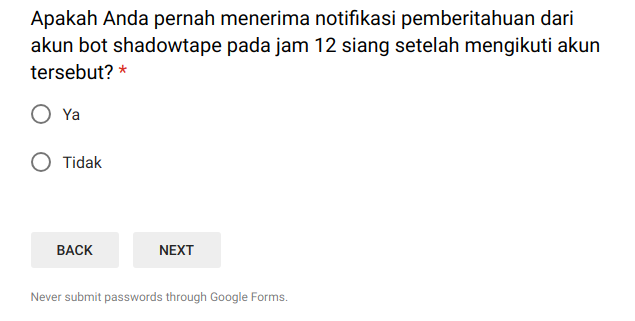
\includegraphics[scale=0.5]{./Survey-Kuesioner/Q1-M2.png}  
	\caption[Kuesioner bagian Mahasiswa pertanyaan ketiga]{Kuesioner bagian Mahasiswa pertanyaan ketiga} 
	\label{fig:q1-m2} 
\end{figure}

Apabila responden memilih jawaban "Ya" pada pertanyaan ketiga (Gambar~\ref{fig:q1-m2}), maka responden akan dialihkan ke pertanyaan keempat (Gambar~\ref{fig:q1-m3}). Apabila responden memilih jawaban "Tidak", maka jawaban responden akan dikirim kepada peneliti.

\begin{figure}[H]
	\centering  
	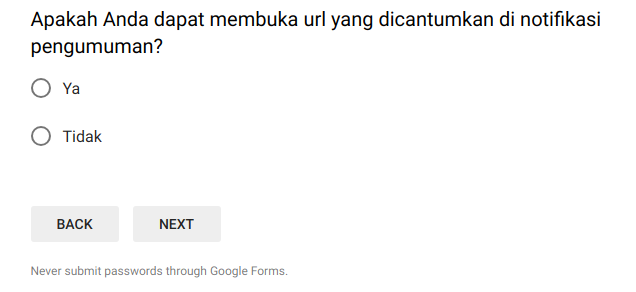
\includegraphics[scale=0.5]{./Survey-Kuesioner/Q1-M3.png}  
	\caption[Kuesioner bagian Mahasiswa pertanyaan keempat]{Kuesioner bagian Mahasiswa pertanyaan keempat} 
	\label{fig:q1-m3} 
\end{figure}

Apabila responden memilih jawaban "Ya" pada pertanyaan keempat (Gambar~\ref{fig:q1-m3}), maka responden akan dialihkan ke pertanyaan kelima (Gambar~\ref{fig:q1-m4}). Apabila responden memilih jawaban "Tidak", maka responden akan dialihkan ke bagian \textit{System Usability Scale} dan Saran (Gambar~\ref{subsec:final}).

\begin{figure}[H]
	\centering  
	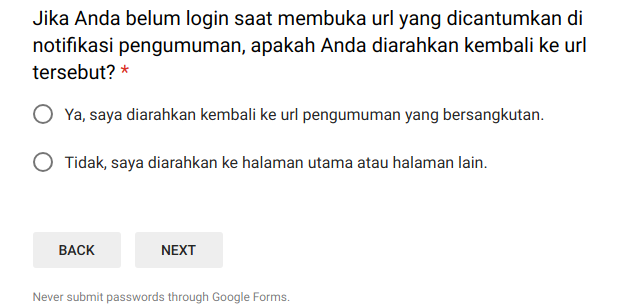
\includegraphics[scale=0.5]{./Survey-Kuesioner/Q1-M4.png}  
	\caption[Kuesioner bagian Mahasiswa pertanyaan kelima]{Kuesioner bagian Mahasiswa pertanyaan kelima} 
	\label{fig:q1-m4} 
\end{figure}

Apapun jawaban responden pada pertanyaan kelima (Gambar~\ref{fig:q1-m4}), responden akan dialihkan ke bagian \textit{System Usability Scale} dan Saran (Gambar~\ref{subsec:final}).

\subsection{\textit{System Usability Scale} dan Saran}
\label{subsec:final}

Bagian ini adalah bagian terakhir dari kuesioner. Bagian ini memiliki 11 pertanyaan yang terdiri dari 10 pertanyaan hasil adaptasi pertanyaan yang ditanyakan saat uji usabilitas dengan metode \textit{System Usability Scale} dan 1 pertanyaan saran. Setelah responden menjawab bagian ini, jawaban responden akan dikirim kepada peneliti. Pertanyaan pada bagian ini ditampilkan pada Gambar~\ref{fig:lq1}, Gambar~\ref{fig:lq2}, dan Gambar~\ref{fig:lq3}.

\begin{figure}[H]
	\centering  
	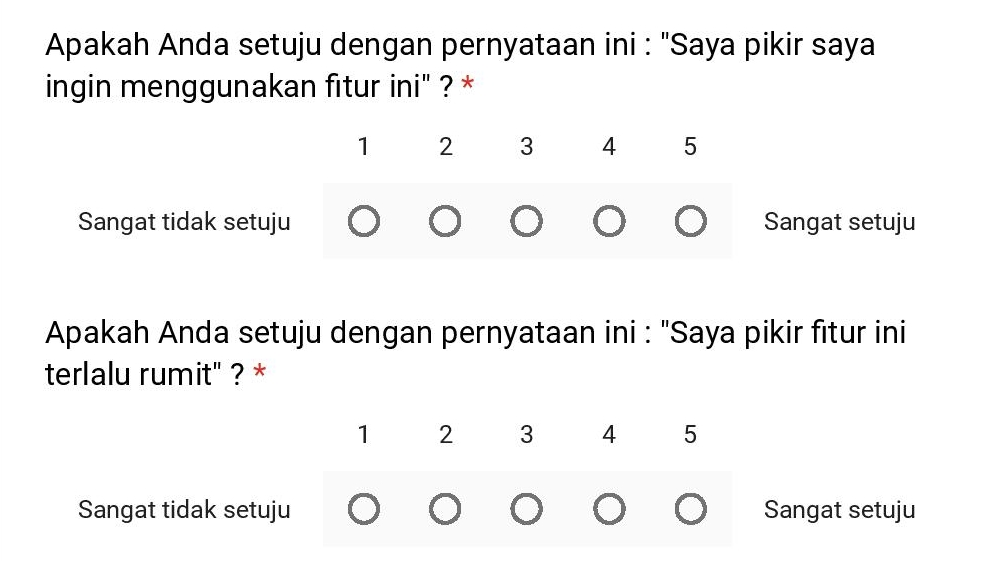
\includegraphics[scale=0.5]{./Survey-Kuesioner/LQ1.jpg} 
	\caption[Kuesioner bagian \textit{System Usability Scale} dan Saran bagian 1]{Kuesioner bagian \textit{System Usability Scale} dan Saran bagian 1} 
	\label{fig:lq1} 
\end{figure}

\begin{figure}[H]
	\centering  
	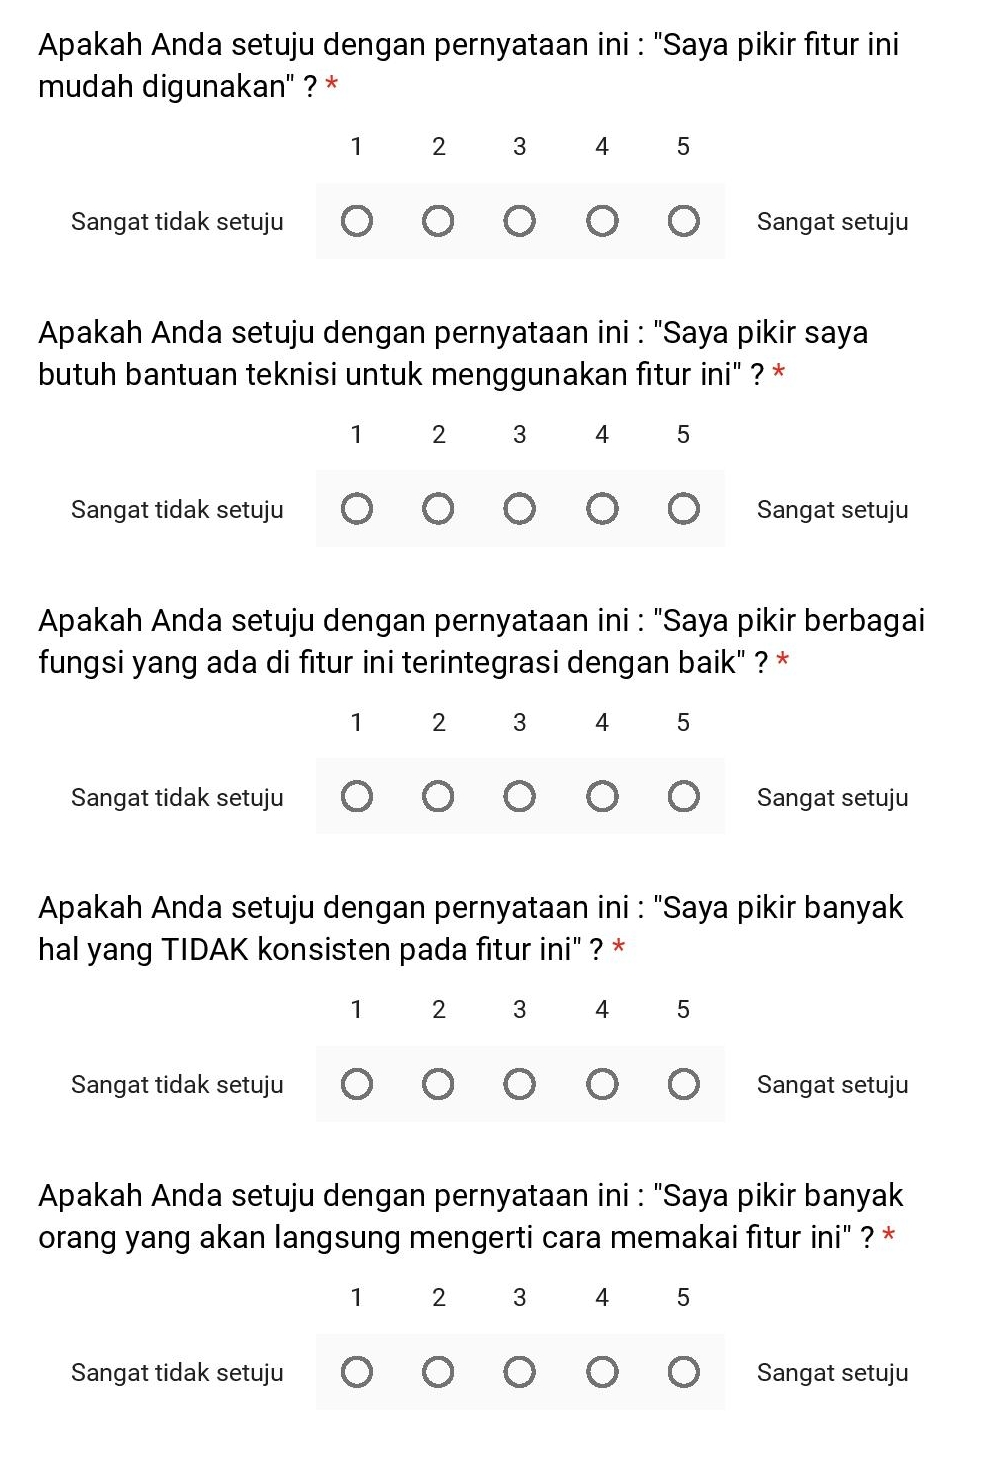
\includegraphics[width=\textwidth]{./Survey-Kuesioner/LQ2.jpg}  
	\caption[Kuesioner bagian \textit{System Usability Scale} dan Saran bagian 2]{Kuesioner bagian \textit{System Usability Scale} dan Saran bagian 2} 
	\label{fig:lq2} 
\end{figure}

\begin{figure}[H]
	\centering  
	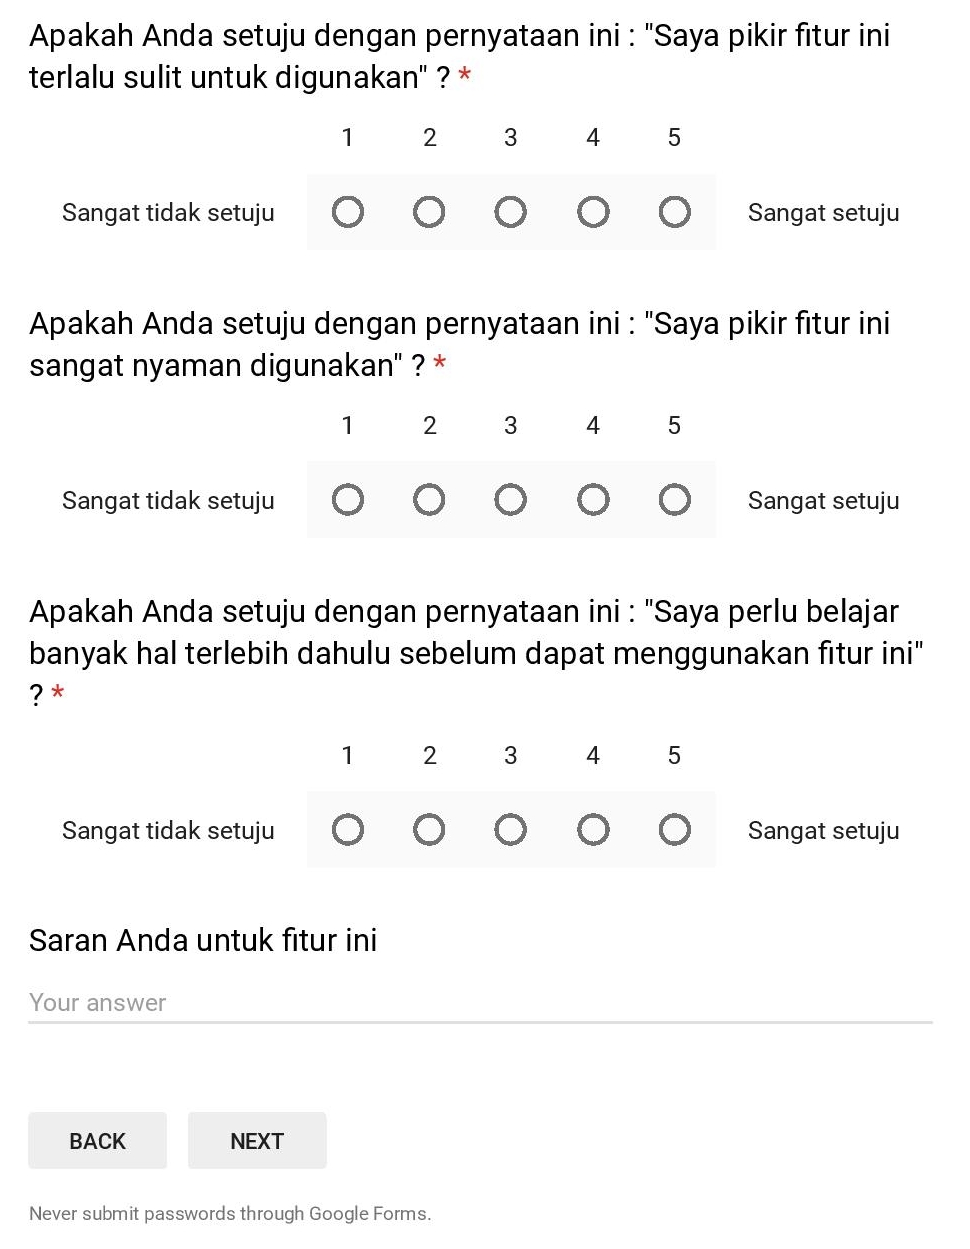
\includegraphics[width=\textwidth]{./Survey-Kuesioner/LQ3.jpg}  
	\caption[Kuesioner bagian \textit{System Usability Scale} dan Saran bagian 3]{Kuesioner bagian \textit{System Usability Scale} dan Saran bagian 3} 
	\label{fig:lq3} 
\end{figure}

\label{sec:full-result-survey}
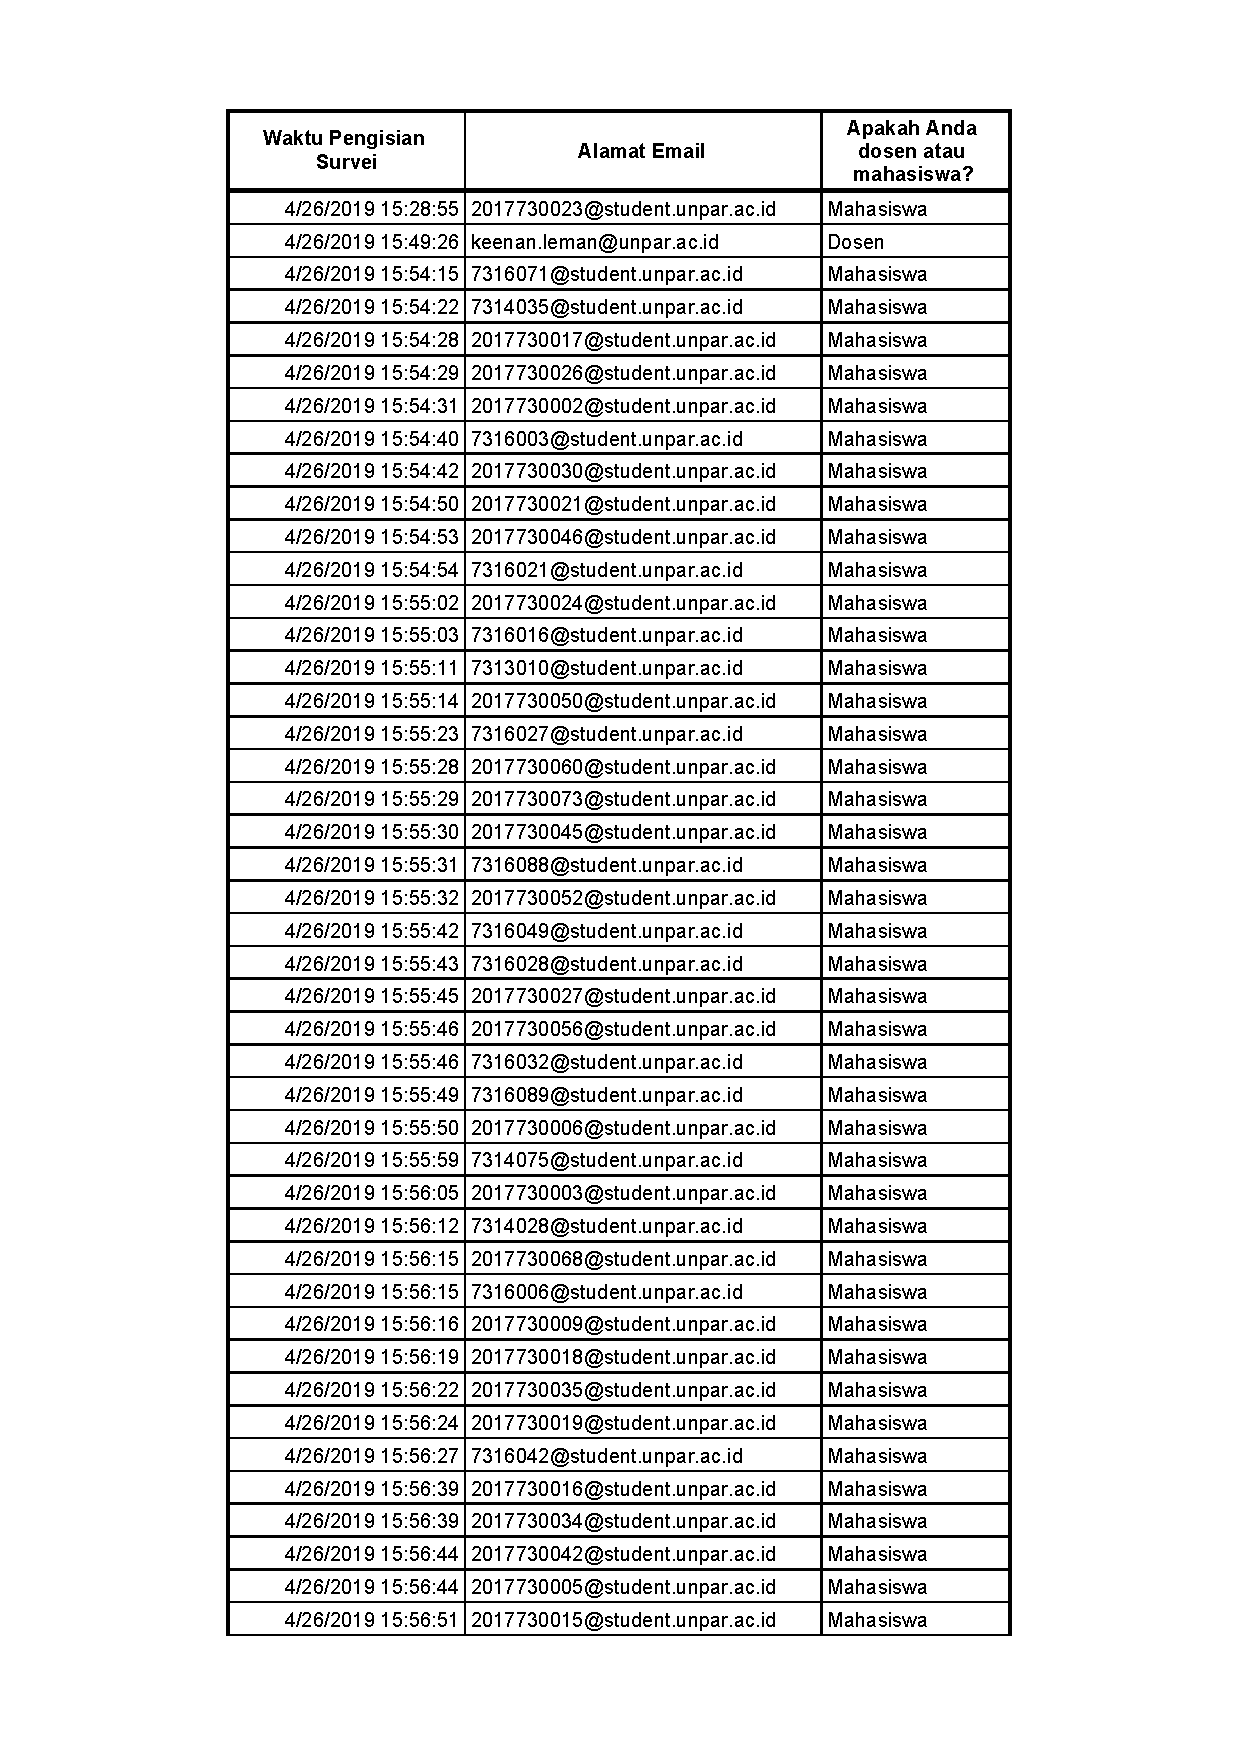
\includepdf[scale=0.8,page=1,pagecommand={\section{Hasil Mentah Kuesioner}}]{./Lampiran/Survey/Survey-DaftarPeserta.pdf}
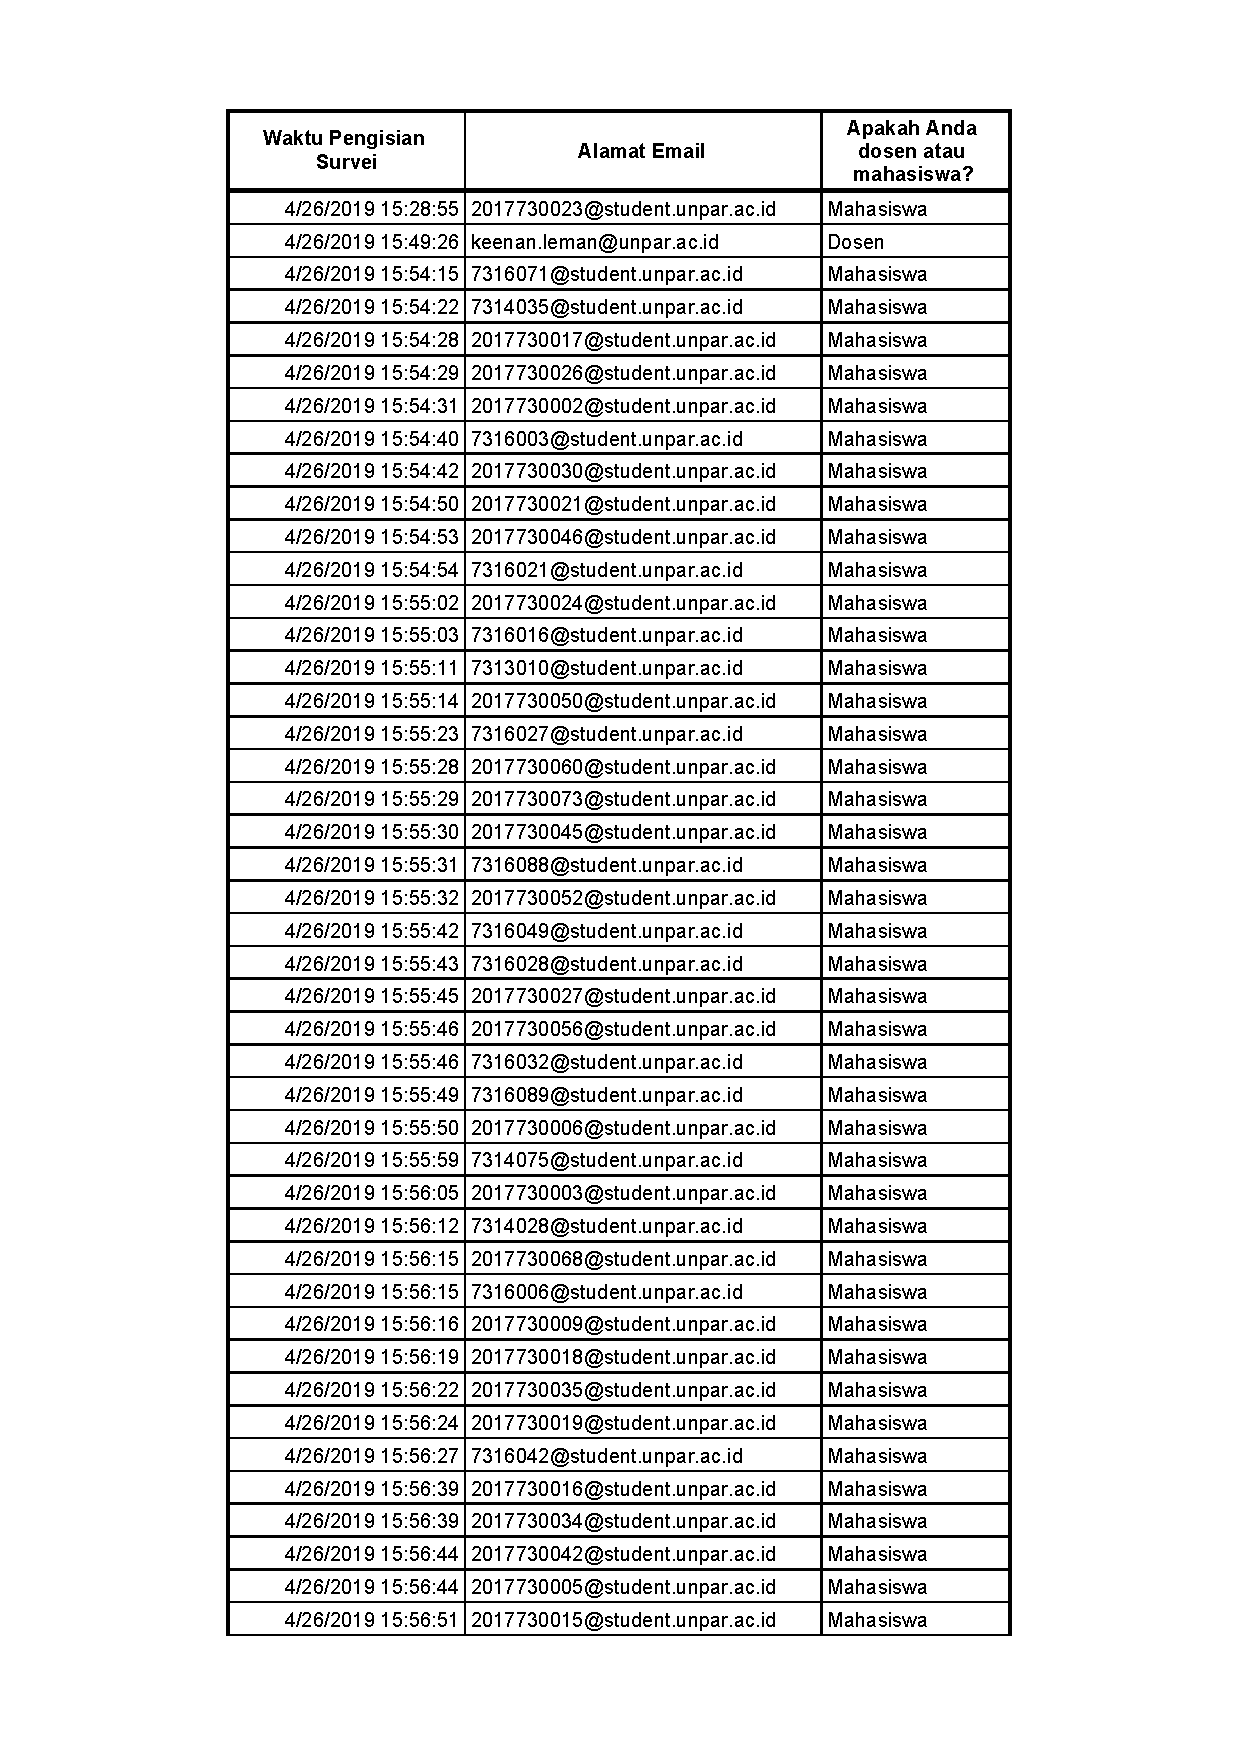
\includepdf[page=2-,pagecommand={},width=\textwidth]{./Lampiran/Survey/Survey-DaftarPeserta.pdf}
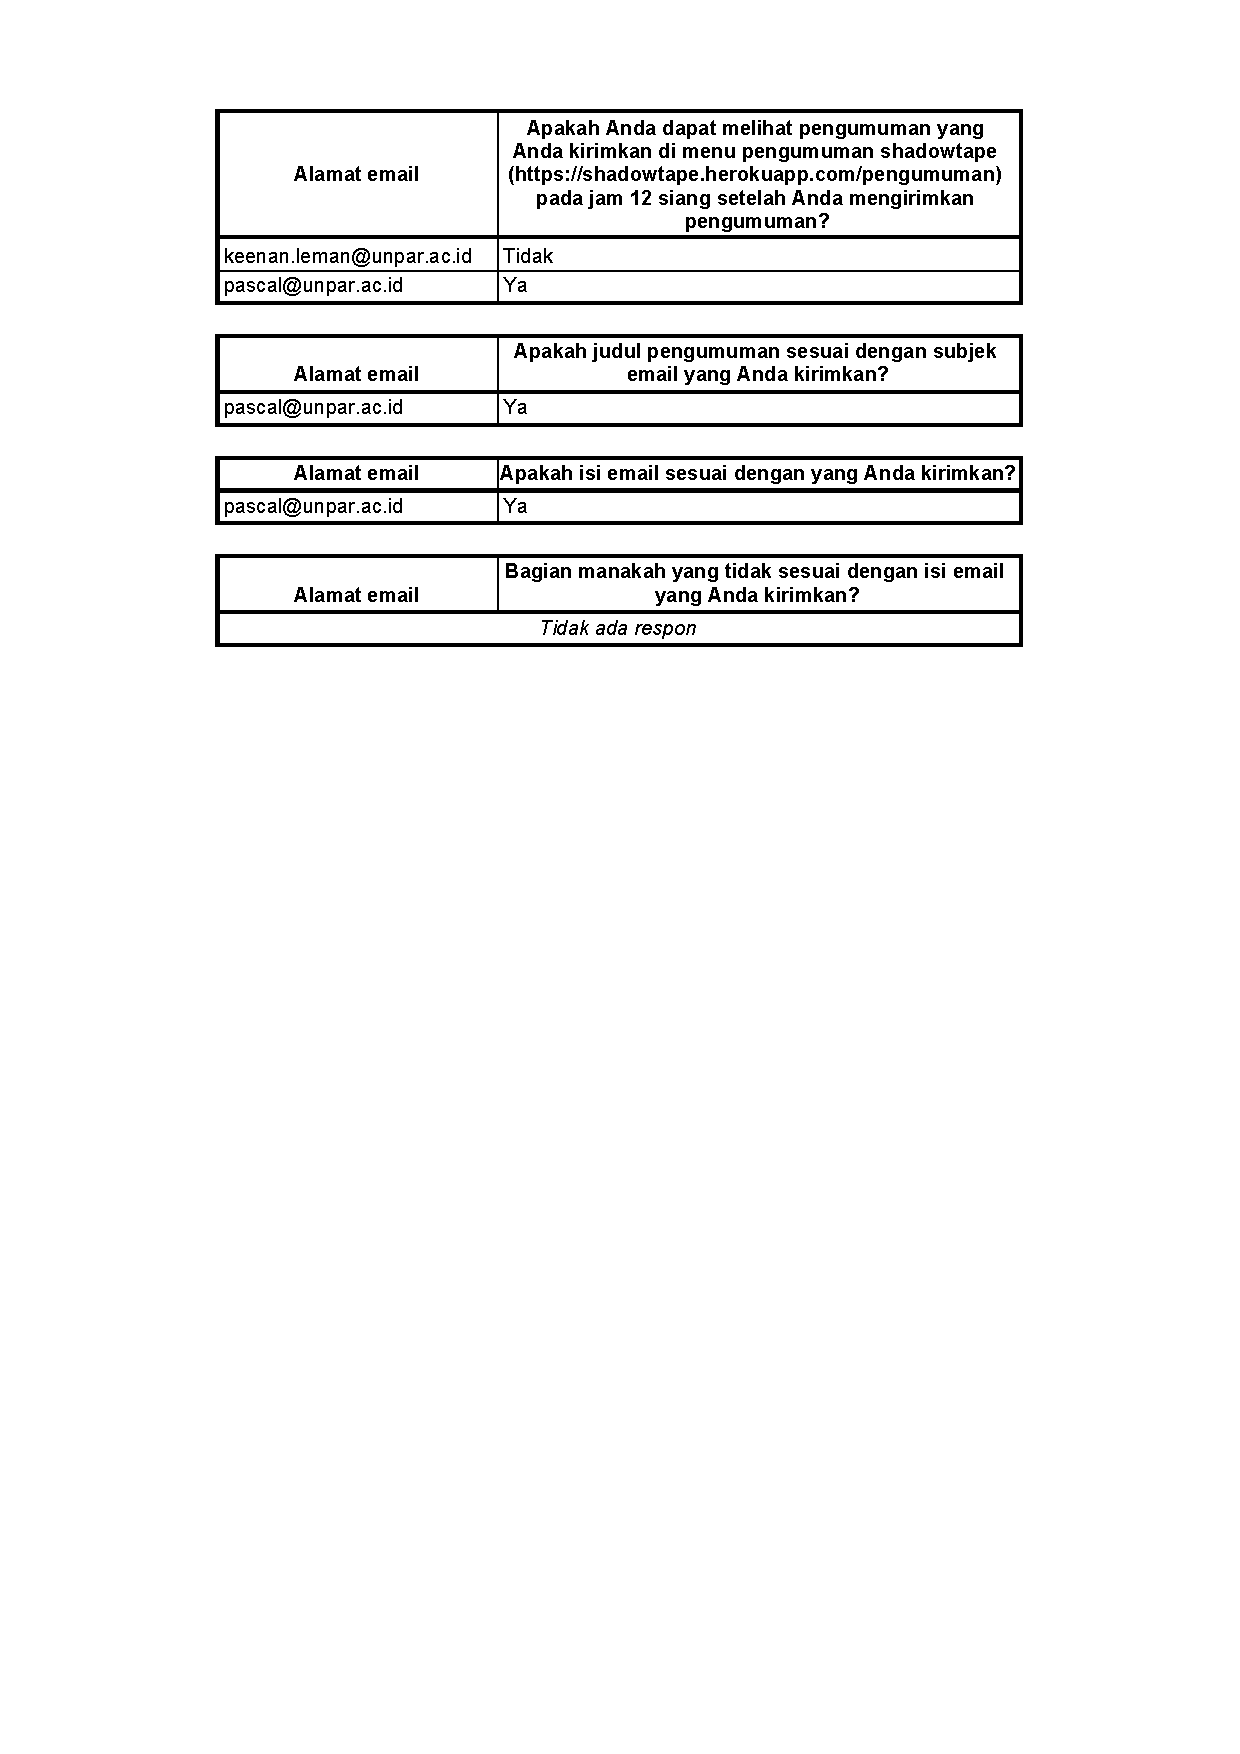
\includepdf[page=-,pagecommand={},width=\textwidth]{./Lampiran/Survey/Survey-Dosen.pdf}
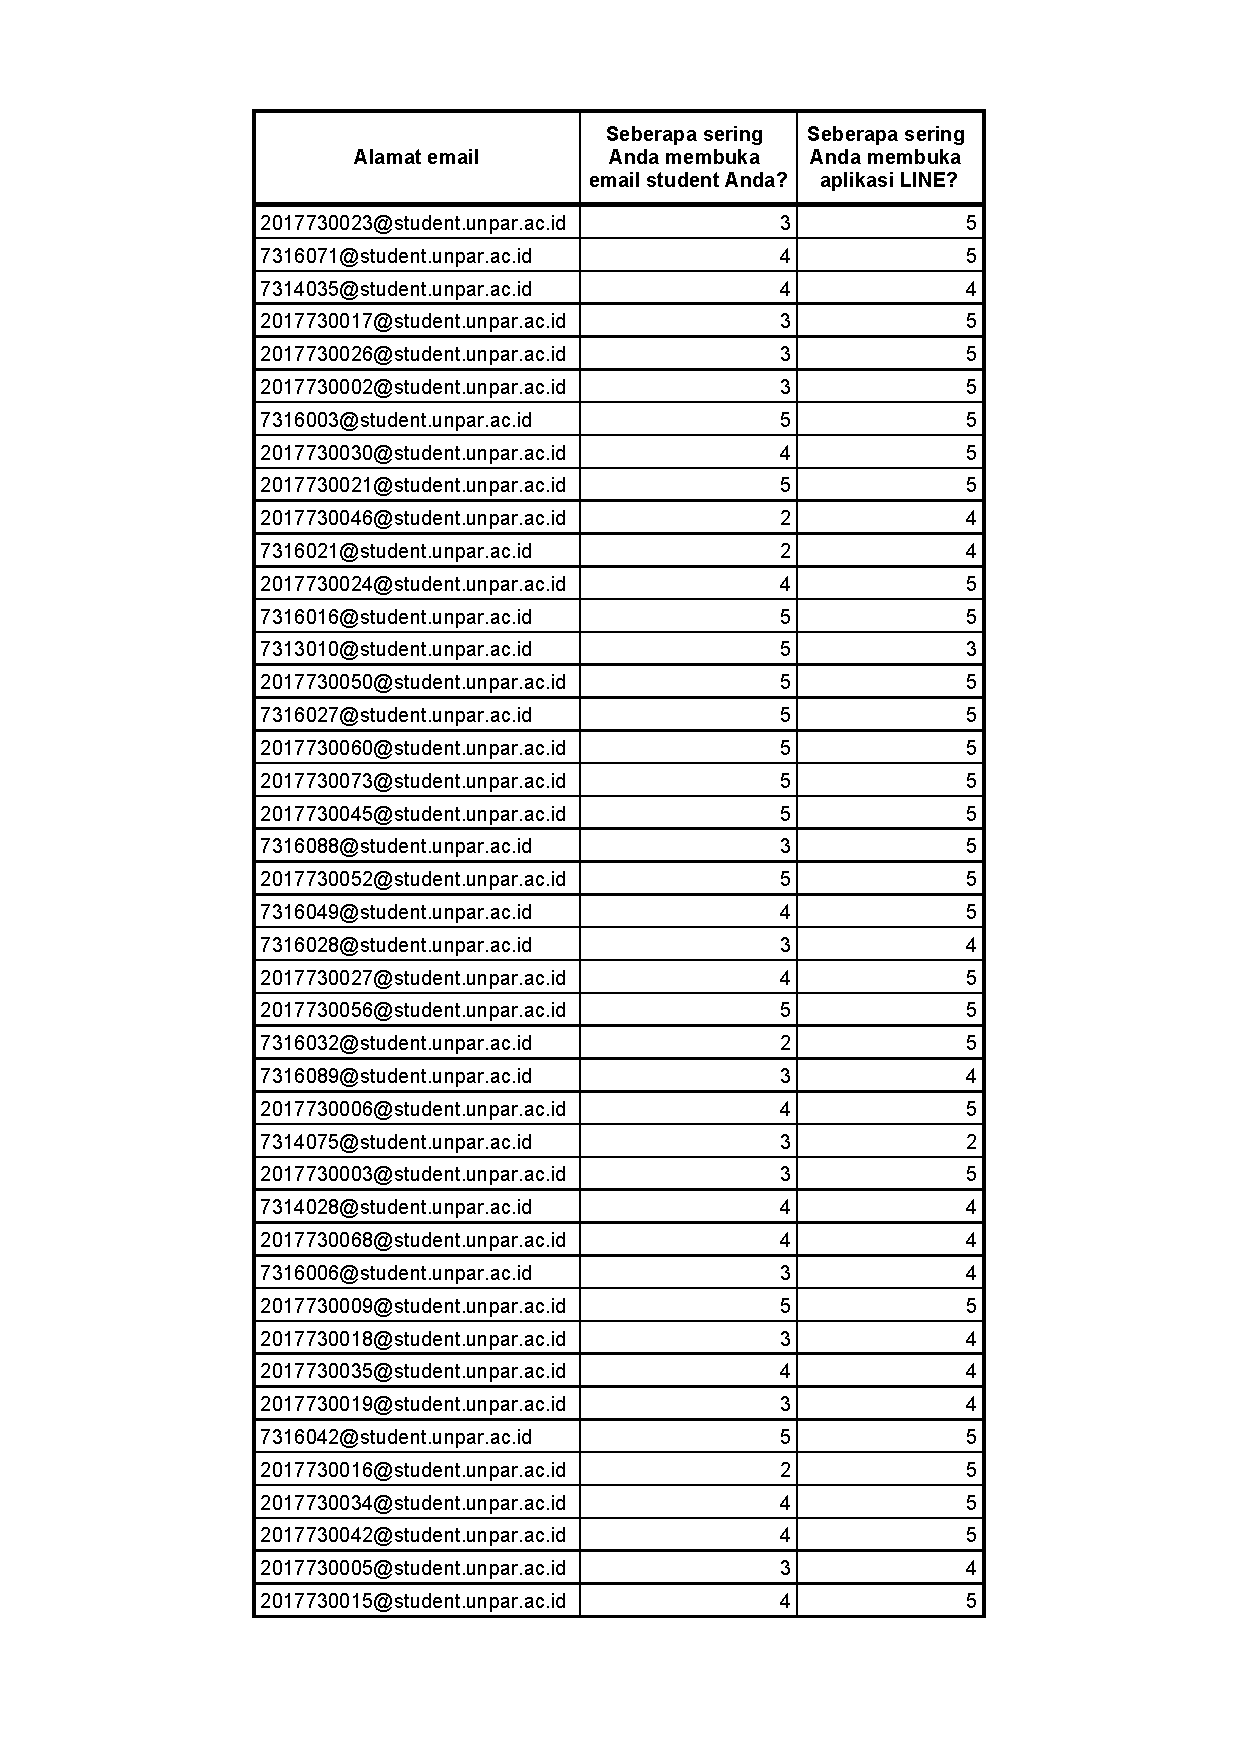
\includepdf[page=-,pagecommand={},width=\textwidth]{./Lampiran/Survey/Survey-PenggunaanEmaildanLINE.pdf}
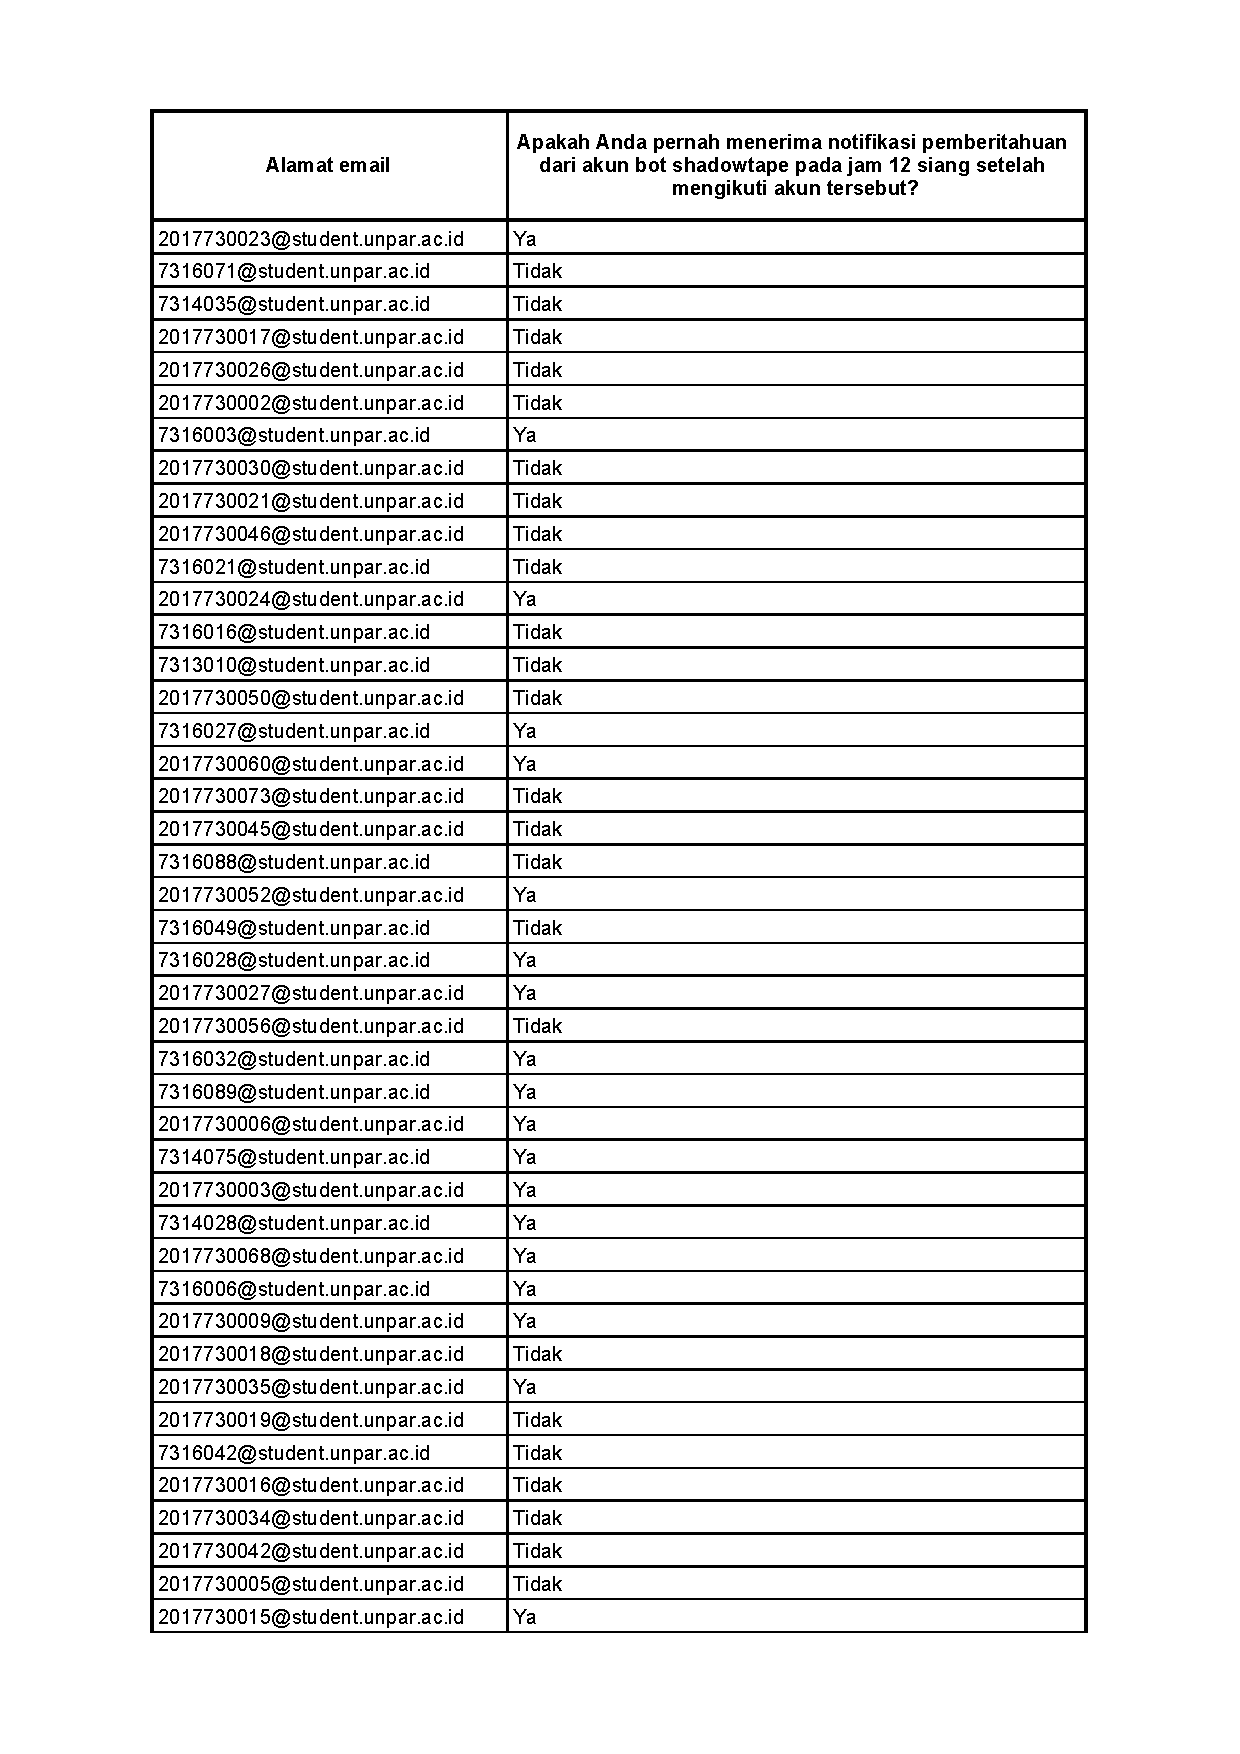
\includepdf[page=-,pagecommand={},width=\textwidth]{./Lampiran/Survey/Survey-TerimaNotifikasiLINE.pdf}
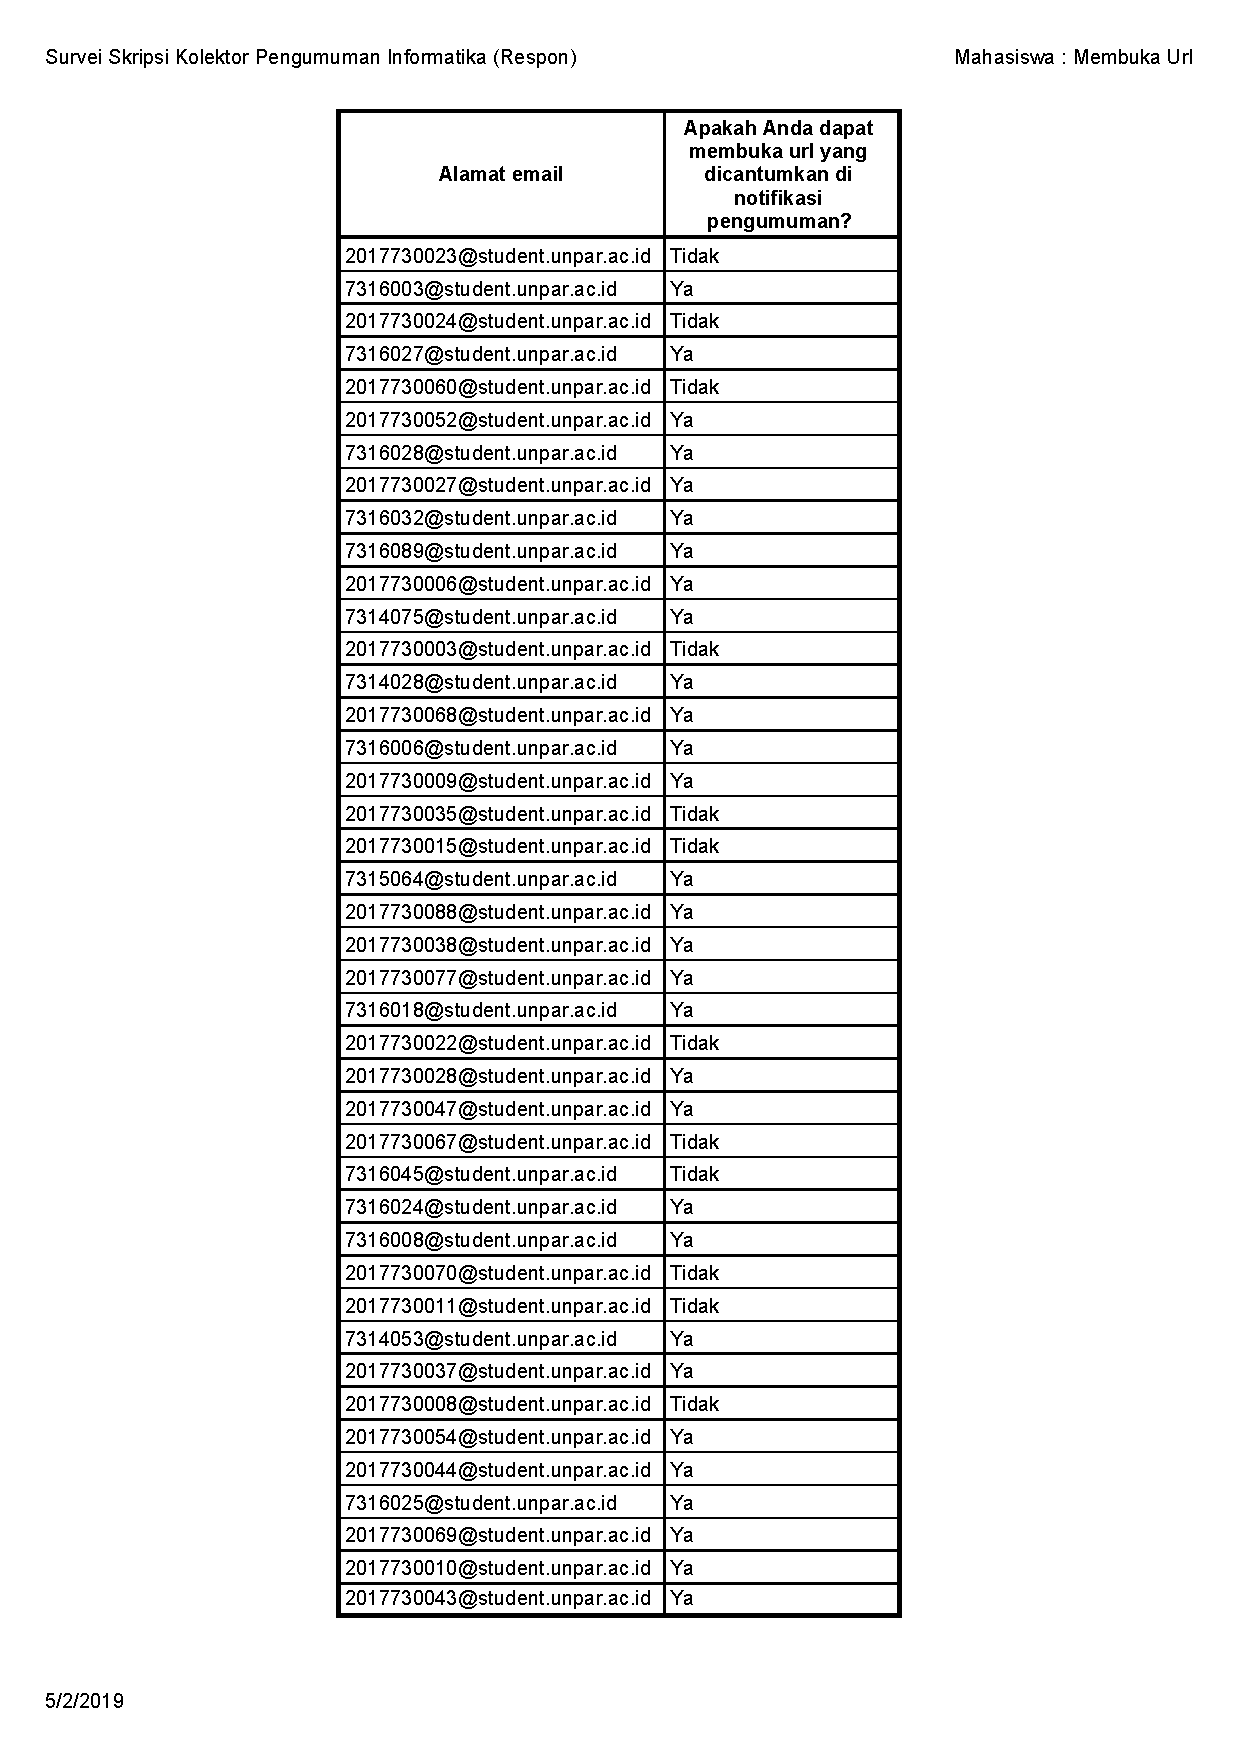
\includepdf[page=-,pagecommand={},width=\textwidth]{./Lampiran/Survey/Survey-Mahasiswa-BukaUrl.pdf}
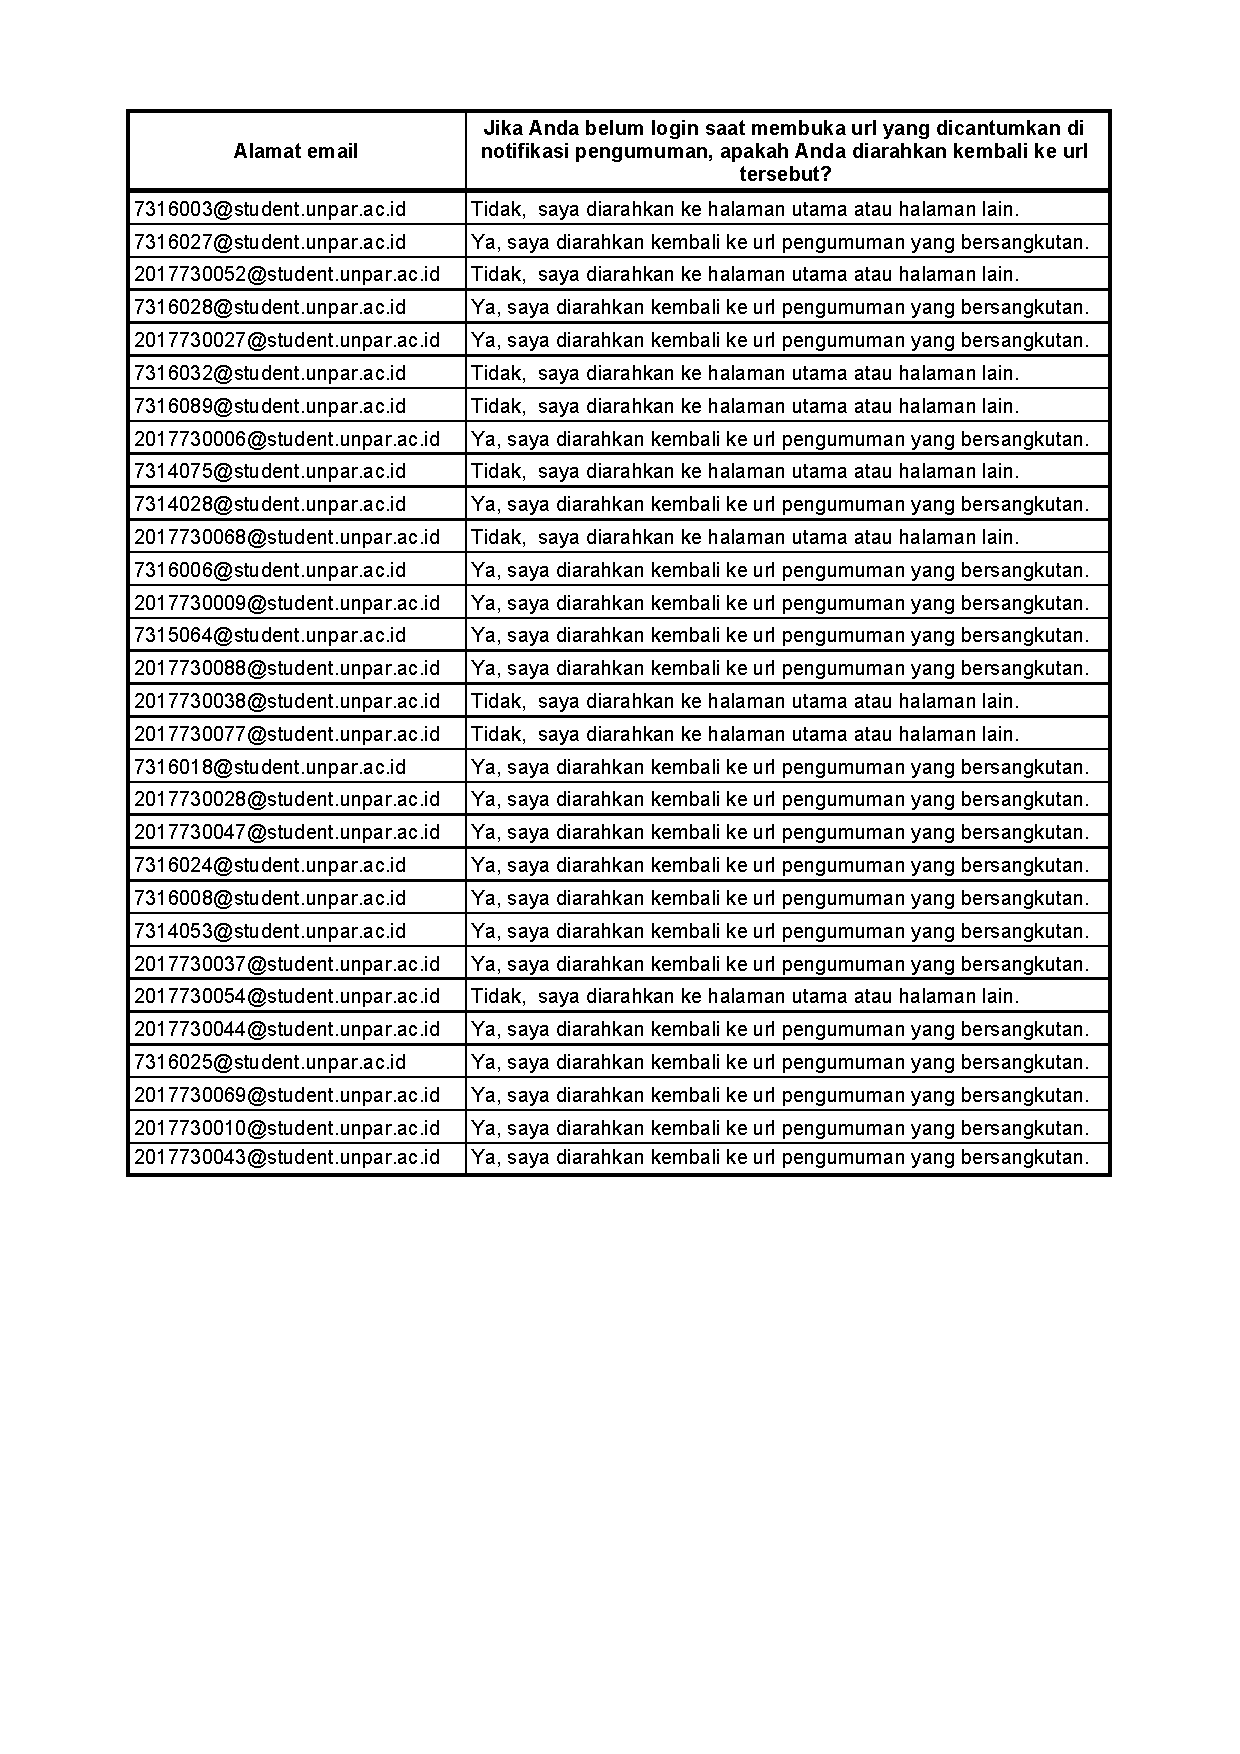
\includepdf[page=-,pagecommand={},width=\textwidth]{./Lampiran/Survey/Survey-Mahasiswa-Redirecturl.pdf}
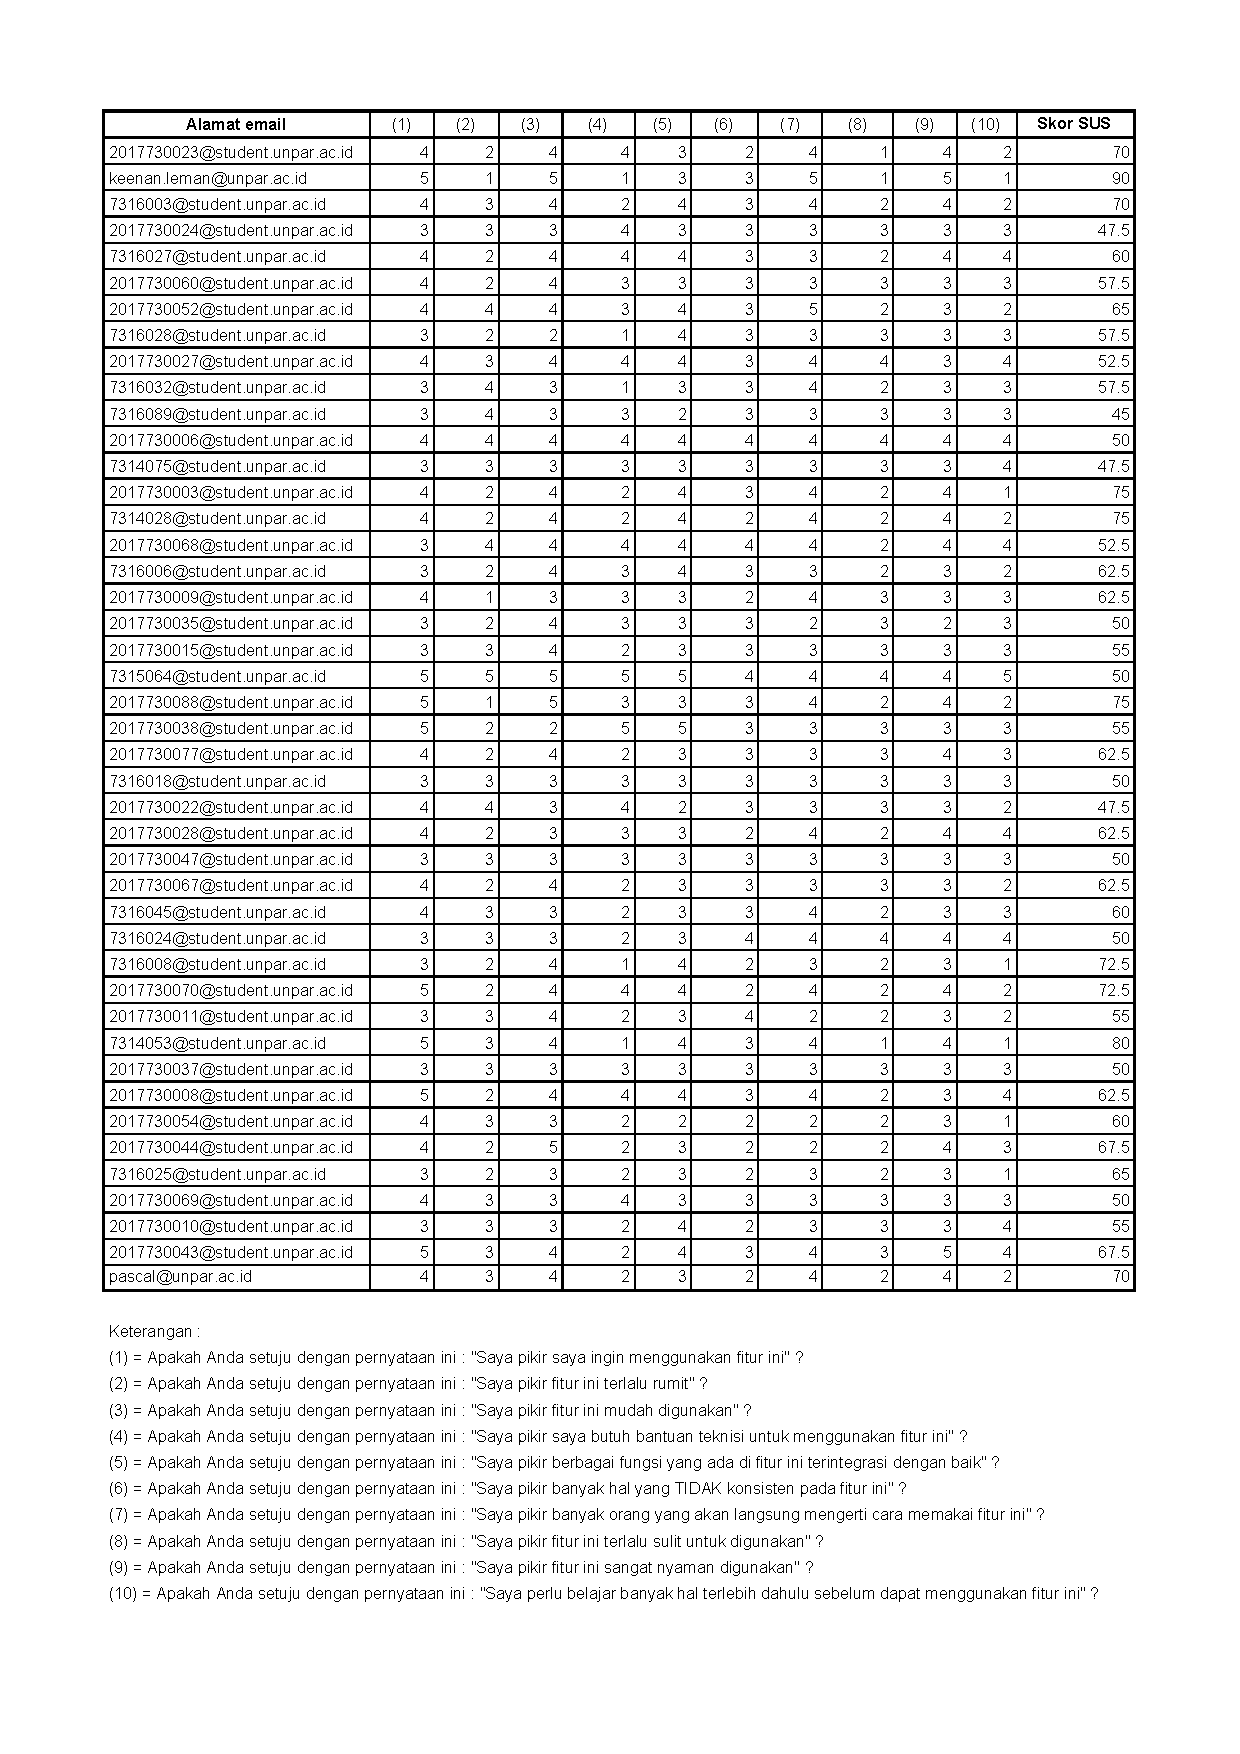
\includepdf[page=-,pagecommand={},width=\textwidth]{./Lampiran/Survey/Survey-SUS.pdf}
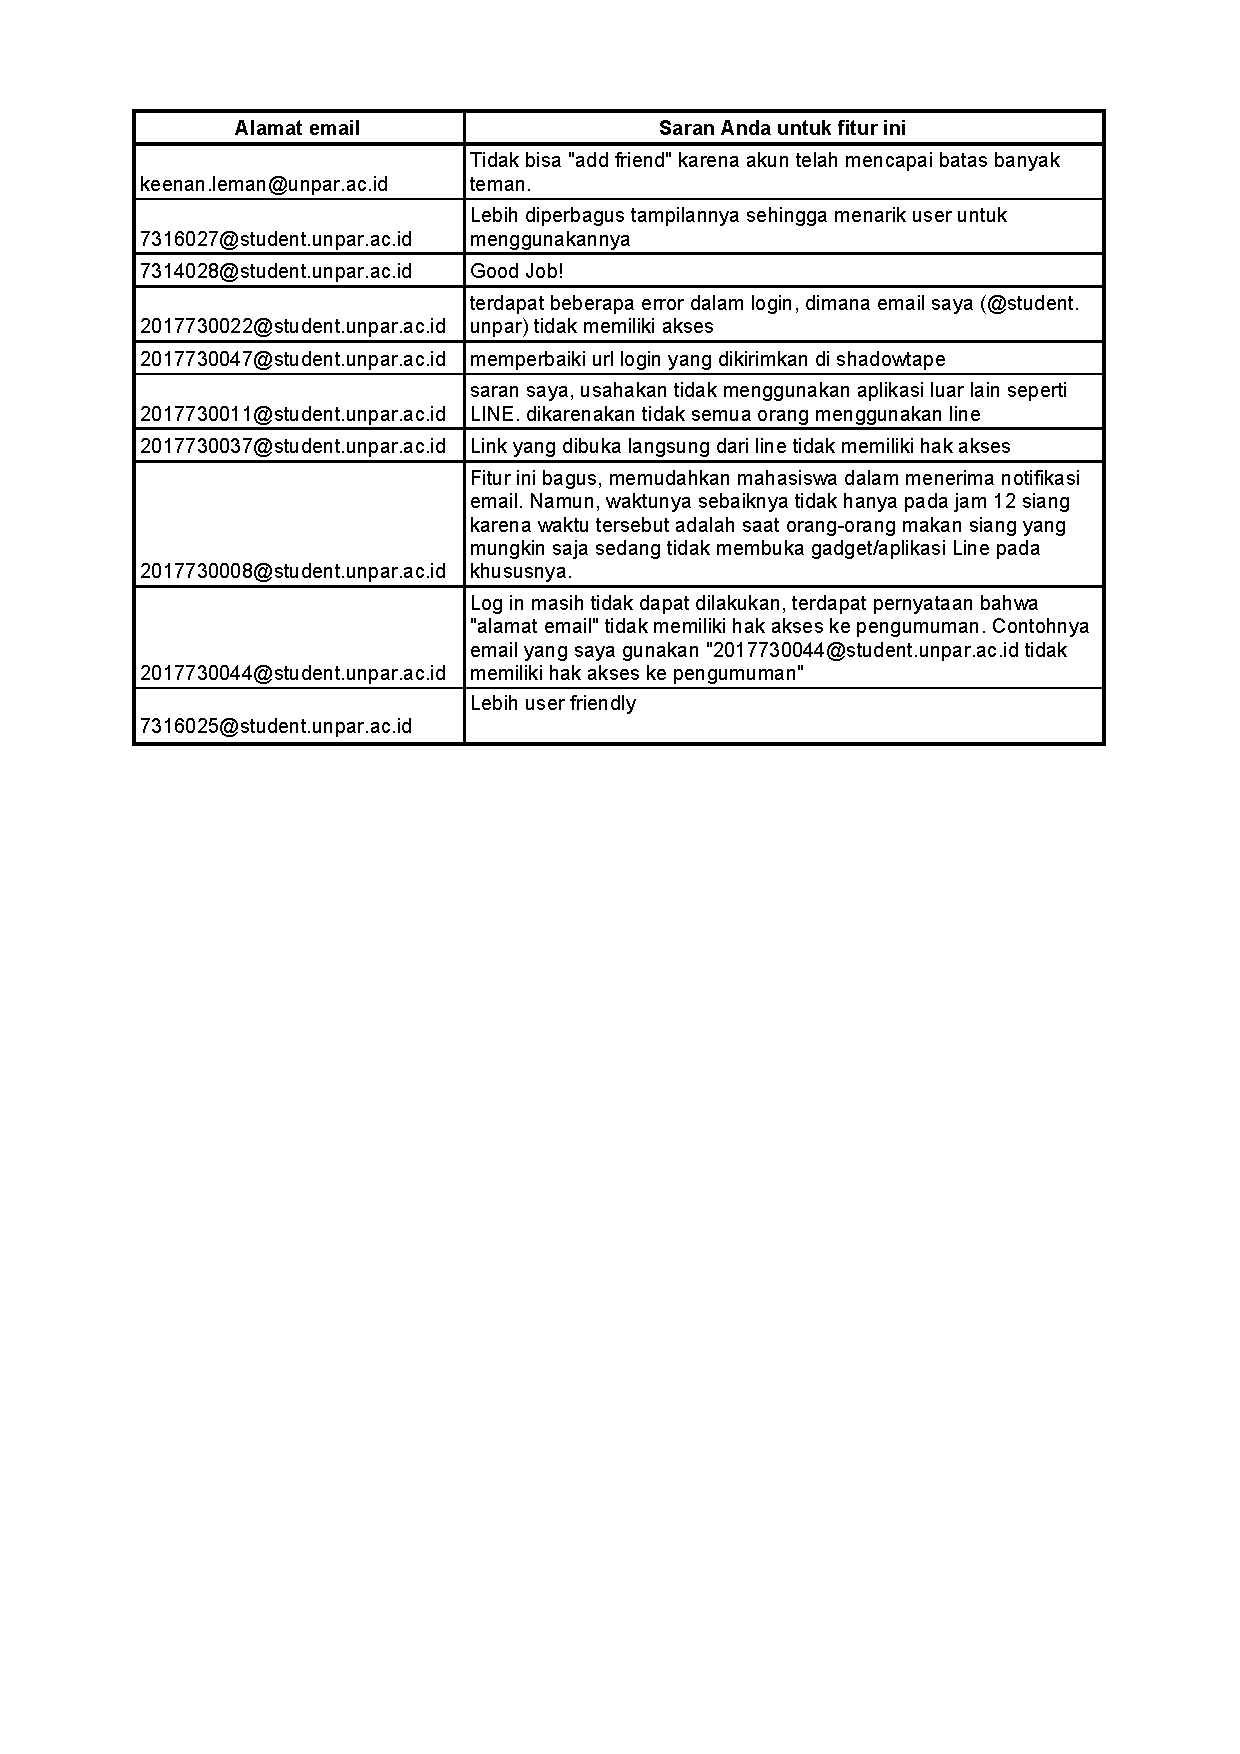
\includepdf[page=-,pagecommand={},width=\textwidth]{./Lampiran/Survey/Survey-Saran.pdf}